\documentclass[../main.tex]{subfiles}
\begin{document}

\chapter{Lecture 8 - 31-03-2020}

$$
|H| < \infty \qquad \hat{h} = argmin \, \hat{\ell}_S \left(h\right) \quad h^* = argmin \, \ell_D\left(h\right)
$$

\blue{minimise risk}
\\\\
\bred{Bias-Variance decomposition}
$$
\ell_d\left(\hat{h}_S\right) = \quad \ell_D\left(\hat{h}_S\right) - \ell_d\left(h^*\right) + \qquad \longrightarrow \red{\textbf{ Variance error $\Rightarrow$ Overfitting}}
$$
$$
\qquad \quad +\,  \ell_d\left(h^+\right) - \ell_d\left(f^*\right) + \qquad \longrightarrow \red{\textbf{ Bias error $\Rightarrow$ Underfitting}}
$$
$$ \qquad \qquad \quad 
+ \, \ell_D\left(f^*\right)\qquad \qquad \quad  \longrightarrow \red{\textbf{ Bayes risk $\Rightarrow$ Unavoidable}} 
$$\\
We state this 
for all algorithm but we studied for ERM.
\\
$$
\ell_D\left(\hat{h}_S\right) \quad \leq \quad \ell_D \left(h^* \right) + \sqrt[]{ \red{\frac{2}{m} \, \ln \, \frac{2\, |H|}{\delta}}} \qquad \textit{with probability at least $1-\delta$ over the draw of $S$}
$$
we want \bred{this} to be small when $m>> \ln|H|$
\\\\
\begin{figure}[h]
    \centering
    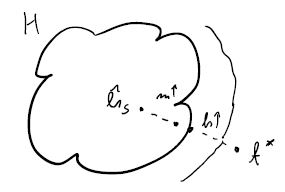
\includegraphics[width=0.5\linewidth]{../img/lez8-img1.JPG}
    \caption{Representation of $\hat{h}$, $h^*$ and $f^*$ }
    %\label{fig:}
\end{figure}\\
Size of model fix, increase $m$ (size of sample) when $m$ is bigger $\longrightarrow$ variance goes down.\\
When $|H|$ $\longrightarrow$ big model will be closer to optimal\\
\begin{itemize}
\item $m$ grows $\Rightarrow$ variance error goes down \qquad (if not overfitting)
\item $|H|$ grows $\Rightarrow$ bias error goes down \qquad (if not underfitting)
\end{itemize}
ERM with $|H| < \infty$
\\
$A$ \qquad $H$ such that $\forall s$ $A(S) \in H$
\\\\
We controlled this event:
$$
\forall h \in H \qquad \hat{\ell}_S(h) - \ell_D \left(h\right) \quad \leq \quad \sqrt[]{\frac{2}{m}\, \ln \, \frac{2\,|H|}{\delta}} 
\qquad 
\textit{ with probability at least $1-\delta$}
$$\\
We assure that training error is a good proxy for the true risk.
\begin{figure}[h]
    \centering
    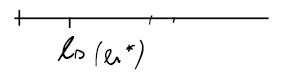
\includegraphics[width=0.5\linewidth]{../img/lez8-img2.JPG}
    \caption{Example}
    %\label{fig:}
\end{figure}\\
\bred{If I do the empirical way(for a specific training set) i get something different.}
\\
\section{The problem of estimating risk in practise}
Test error is a good estimate for a risk, provided $\frac{1}{\sqrt[]{n}}$ is small\\\\
It’s usually good to take a small test set.\\
$80/20$ big data, if low data better to look at good estimate...=??\\
Usually small test set is still ok\\\\
Typically we are not given the predictor, instead we start from a learning
algorithm. It’s true that A has parameter (how many nodes for a tree classifier
for example).\\
In general, if I have parameters then i get a set of different classifier
Imaging Algorithm that has parameter $\theta$:
$$ 
A \qquad  \{ A_{\theta}: \theta \in \Theta \} \qquad
A_{\theta} \left(S\right) = \hat{h}_S
$$
$\barra{E} \left[ \ell_D \left( A_\theta \left(S \right) \right) \right]
$ \qquad \bred{typically averaged over $S$ of size $m$ for fixed $m$}
\\\\In general you may also be interest looking at the best choice of parameter for
your algorithm:
Suppose now that i want to look at mini sing the risk with the respect to the
choice of the parameter\\\\
$\barra{E} \left[ \, min \, \ell_D \left( A_\theta \left(S \right) \right) \right]
$ \quad i want to choose parameter that minimise risk running algorithm on training set.
\\\\
I would like to choose best possible value for my parameter k in the k-NN and
i want to estimate the risk.\\
$\theta$ can be a set of parameters (so more than 1 parameter), so theta are
the \textbf{hyper parameters of A}.\\
In general this parameter are the choices that algorithm that can make:
parameter that define a classifier (example nodes and test in the internal
nodes and label in the leaves)\\\\
\bred{Hyper parameters} are not determined by the training set $\rightarrow$ chosen
before the training set.\\
I fix $k$ for $\knn$ and I choose an upper bound of number of nodes after the
training set is given.\\
So, some parameters are given after training set is given and some parameter
fixed before.\\
Now the idea is that parameter are determined after training set is given, while
hyper parameters are given before training set to get then a predictor.\\
I have a family of algorithms, so I choose a hyper parameters to get a one
algorithm.\\
Most algorithm are given as family. We have first decide hyper parameters not
determined on the training set.\\
One way to move is to take you dataset and the split that in 3 parts:
\begin{itemize}
\item Training set
\item Development (or validation) test
\item Test sets
\end{itemize}
There should not be a leak of information between test and train and
development.\\
We get family of algorithm, train with train set and then use dev set to test the
parameter and choice the parameters.
Once i found the parameter I retrain the algorithm with a part of train and dev
set to being then tested.
\\
\bred{Development set is like a fake test set } $\rightarrow$ it usefull to choose parameters.
\\
Algorithm steps:
\begin{enumerate}
\item  Train $A_\theta$ on training set for each $\theta \in \Theta $ (\bred{grid search}) 
\item Find $\theta$ such that $\hat{h}= A_{\hat{\theta}}\left(S\right)$ \, minimise developement error
\item Train $A_{\hat{\theta}}$ on training $+$ development set
\item Test resulting predictor on test set
\end{enumerate}
(There's theory about this but it's difficult and we are not going to do that)
\\\\
It’s heuristic and kinda simple to do. This technics work for every learning
algorithm.\\
One parameter: grid on this\\
Two parameters ecc..\\
\textbf{It’s quadratic!}\\
\bred{Good learning algorithm should have small number of hyperparameters.}

\section{Cross-validation}

Solving an easier problem: suppose you have a dataset and what you do is
that you can choose training set and test set.\\
Algorithm $A$ with no hyper parameters and we would like to check how good is
the predictor: how good can $A$ be? $A$ is good if the predictor that generate has
low risk.\\
I split dataset in training and test set.
\begin{figure}[h]
    \centering
    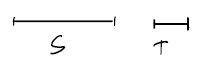
\includegraphics[width=0.5\linewidth]{../img/lez8-img3.JPG}
    \caption{Splitting test and training set}
    %\label{fig:}
\end{figure}
$$
h = A\left(A\right) \qquad \hat{\ell}_{S'}\left(h\right) \approx \ell_D\left(h\right)
$$
I can use Cross-validation! (CV). It helps estimate the risk.
$$
\bred{CV:} \qquad \barra{E}\left[ \ell_D \left(A\left(S \right) \right) \right]
$$
I would like to average .... \\
How do i do this estimate? Super easy, take my data assuming CV as
parameter not of the algorithm A, but intrinsic to cross validation.\\
Parameter k-fold CV typically $k = 5$ or $10$.\\
What do you do ? If i take a specific training set, i got a ruff estimate of A.
I shouldn’t split one but several time.\\
There are different way but he give us another:\\
\textbf{split data in k folds randomly!}
\begin{figure}[h]
    \centering
    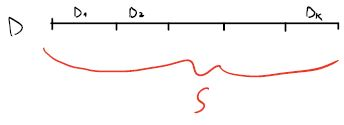
\includegraphics[width=0.6\linewidth]{../img/lez8-img4.JPG}
    \caption{K-folds}
    %\label{fig:}
\end{figure}\\
For each $k$ we define $S^{(k)}
 \qquad \bred{take out k-st D}$
$$
S^{(k)} = S\backslash D_k
$$
$$
S^{(1)} = D_2 \cup D_3 \cup ...\cup D_k
$$
$$
S^{(2)} = D_1 \cup D_3 \cup ... \cup D_k
$$
For each $k-1, ... k$ \bred{folds} \qquad $S^{(k)}$ training part and $D_k$ test part
$$
h_K = A \left( S^{(k)} \right) \qquad \hat{\ell}_{DK} \left(h_K\right) = \frac{k}{m} \, \sum_{ (x,y) \in D_k}{} \ell \left( y, h_K\left( x \right) \right ) 
$$
Repeat the procedure for $k = 1 ... k$ \quad get $h_1, ... , h_k$
\\
$$
Compute \qquad \frac{1}{k} \cdot \sum_{k=1}^{K} \hat{\ell}_{DK} \left(h_k\right)
$$
where $CV$ is $\barra{E}\left[ \ell_D \left(A\left(S \right) \right) \right]$ and this is called ..... ---MANCA ---  Estimate
\\\\
It’s used a lot!\\
You get data from internet, then what to do? I want to try an algorithm, try $\knn$ so you do Cross validation and will give you the risk.\\
In some other cases you get a splitted dataset in training and testing set.
You don’t use CV since the dataset is already splitted in training and test.

\section{Nested cross validation}
The use of CV to solve the hyper parameters choice problem.
If you are given test and training set you can solve splitting in training set and
dev set.\\
Suppose not given train and test, you can assign arbitrary .....\\
Now the idea: you give me a way to optimise splitting training set and test set
and then avoiding using a ...\\
\textbf{This is what cross validation is doing.}
\begin{figure}[h]
    \centering
    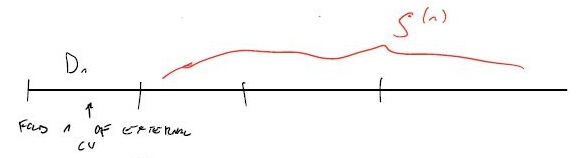
\includegraphics[width=0.8\linewidth]{../img/lez8-img5.JPG}
    \caption{Nested Cross Validation}
    %\label{fig:}
\end{figure}\\
$ \{ A_\theta : \theta \in \Theta \}$
which i run in each fold?
\\
The idea is \bred{running interval CV for the folds}\\
I have fold $D_1$ and $S(1)$ and i perform external validation, then i run internal
CV in $S(1)$.\\
On each training part of the external CV, run a internal CV for each $A_\theta$.
\\When $\theta \in $ grid ($\Theta$):
\begin{itemize}
\item I have a CV-estimate and for each $A_\theta$ pick the $\theta$ with best CV-estimate
\item Run $A_{\hat{\theta}}$ on the entire training part of current external fold
\end{itemize}
\textbf{Basically what I’m choosing the best hyper parameter on each fold of the
external CV.}\\
External CV is not testing $A_{\hat{\theta}}$ for a given $\hat{\theta} \in \Theta$
\\
I am not measuring a goodness of predictor generate by algorithm for given
value of hyper parameters but what I’m estimating is the average risk of the
predictor output by learning algorithm when hyper parameters are optimise on
the training set. This optimisation on training set is done into a internal CV. To
avoid be depend i run and external CV.\\
Many platform like sklearn allow you to do that in two lines of code. So i can
specify the grid, predictor, number of falls for internal and external.
It took a bit but that’s it in in two lines of code\\
Cross validation can be done in every order of $D_1$ or $D_2$ or $D_k$. So doesn’t
matter the order we start fold D2 or D1.
\end{document}